%!TEX root = ../template.tex
%%%%%%%%%%%%%%%%%%%%%%%%%%%%%%%%%%%%%%%%%%%%%%%%%%%%%%%%%%%%%%%%%%%%
%% chapter5.tex
%% NOVA thesis document file
%%
%% Chapter with lots of dummy text
%%%%%%%%%%%%%%%%%%%%%%%%%%%%%%%%%%%%%%%%%%%%%%%%%%%%%%%%%%%%%%%%%%%%
\chapter{Evaluation}
\label{cha:evaluation}

%\textbf{TOPICS :}
%\begin{itemize}
%	\item Benchmark the iCBD-Replication Module
%	\item Assert the performance gained by storing iMI closer to client workstations
%\end{itemize}

The following chapter reports the experimental work performed in order to study both the performance of the implemented replication module and the executability and the performance improvements to the introduction of a cache server role in the iCBD platform.

É de notar que a validade funcional foi testada durante todo o processo de desenvolvimento, notando-se que todos os componentes apresentados encontram-se funcionais.
Este capitulo mostra 

The chapter is divided into the following sections:

\begin{description}
    %
    \item [Section~\ref{}] .
    %
    \item [Section~\ref{}] ..
    %
\end{description}


%%-------------------------------------------------------------------
%%	5. - Motivation
%%-------------------------------------------------------------------
%\section{Motivation}
%\label{sec:eval_motivation}

%https://stackoverflow.com/questions/1198691/testing-io-performance-in-linux
%https://dl.acm.org/citation.cfm?id=1367829.1367831

%https://github.com/axboe/fio
%https://github.com/giantswarm/filesystem-benchmark

%%-------------------------------------------------------------------
%%	5. - Metodology
%%-------------------------------------------------------------------
\section{Metodology}
\label{sec:eval_method}

Unless stated otherwise, all tests were executed ten times removing the best and worst result. The final result is the average of the remaining values. 
%Throughput results are presented in Transactions per Minute (TPM).


%%-------------------------------------------------------------------
%%	5. - Experimental Setup
%%-------------------------------------------------------------------
\section{Experimental Setup}
\label{sec:eval_exp_setup}

\begin{table}[htpb]
\centering
\begin{tabular}{lcc}
%\hline
                             & \textbf{FCT NOVA}          & \textbf{Reditus}              \\ \hline
\textit{\textbf{Servers}}    & 2x HPE ProLiant DL380 Gen9 & 2 x HPE ProLiant DL380 Gen9   \\
\textit{\textbf{Switch}}     & HPE Flexfabric 5700 jg898a & HPE Flexfabric 5700 jg898a    \\
\textit{\textbf{Disk Array}} & HPE MSA 2040 SAN Storage   & N/A - (Storage on the Server) \\
\textit{\textbf{Networking}} & 10 Gbps (between servers)  & 10 Gbps (between servers)     \\ \hline
\end{tabular}
\caption{Physical infrastructure of the FCT NOVA and SolidNetworks sites}
\end{table}




%%-------------------------------------------------------------------
%%	5. - Replication Service Benchmark
%%-------------------------------------------------------------------
\section{Replication Service Benchmark}
\label{sec:eval_rep_bench}

%\textbf{TOPICS :}
%\begin{itemize}
%	\item Replication with rsync (100 / 1000 mbps)
%	\item Replication with iCBD-Replication - Plain Sockets and No Compression (100 / 1000 mbps)
%	\item Replication with iCBD-Replication - Plain Sockets and LZ4 Compression (100 / 1000 mbps)
%	\item Replication with iCBD-Replication - Plain Sockets and zlib Compression (100 / 1000 mbps)
%	\item Replication with iCBD-Replication - Plain Sockets and snappy Compression (100 / 1000 mbps)
%	\item Replication with iCBD-Replication - SSH and No Compression (100 / 1000 mbps)
%\end{itemize}

%https://stackoverflow.com/questions/5357601/whats-the-difference-between-unit-tests-and-integration-tests

% Unit Test Python
%https://docs.python.org/2/library/unittest.html

%Memory profile of the module
%https://pypi.python.org/pypi/memory_profiler




%%-------------------------------------------------------------------
%%	5. - Cache Server Performance Benchmark
%%-------------------------------------------------------------------
\section{Cache Server Performance Benchmark}
\label{sub:eval_cache_bench}

\begin{figure}[htbp]
	\centering
	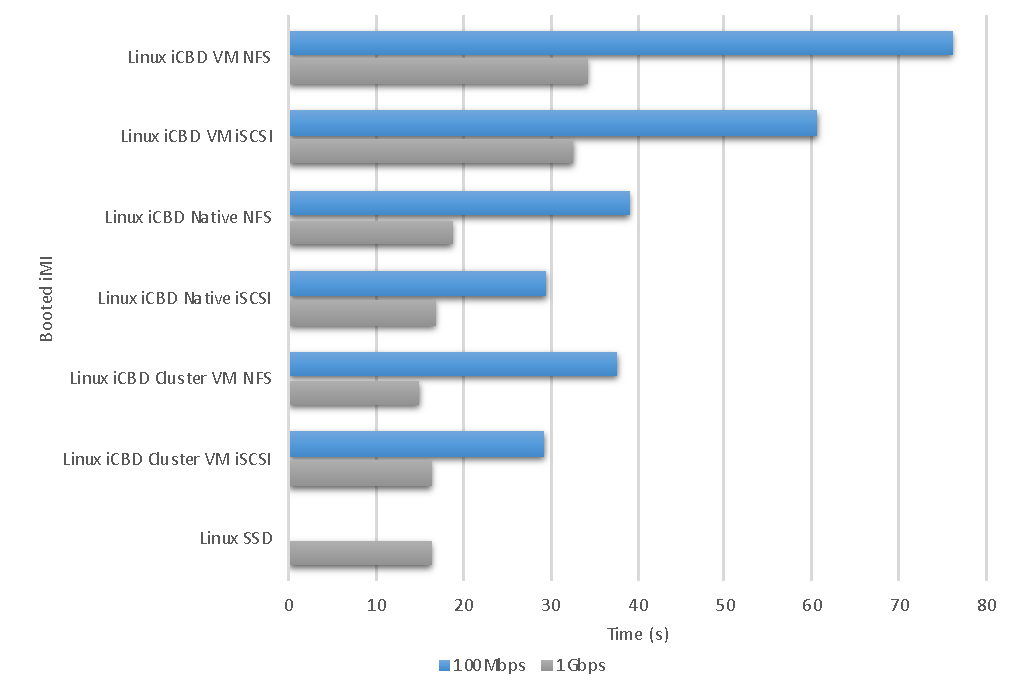
\includegraphics[height=4in]{cap5_secboot_imgs}
	\caption{Boot time from iCBD-imgs VM in a five workstation sequential boot scenario}
	\label{fig:boot_imgs}
\end{figure}

\begin{figure}[htbp]
	\centering
	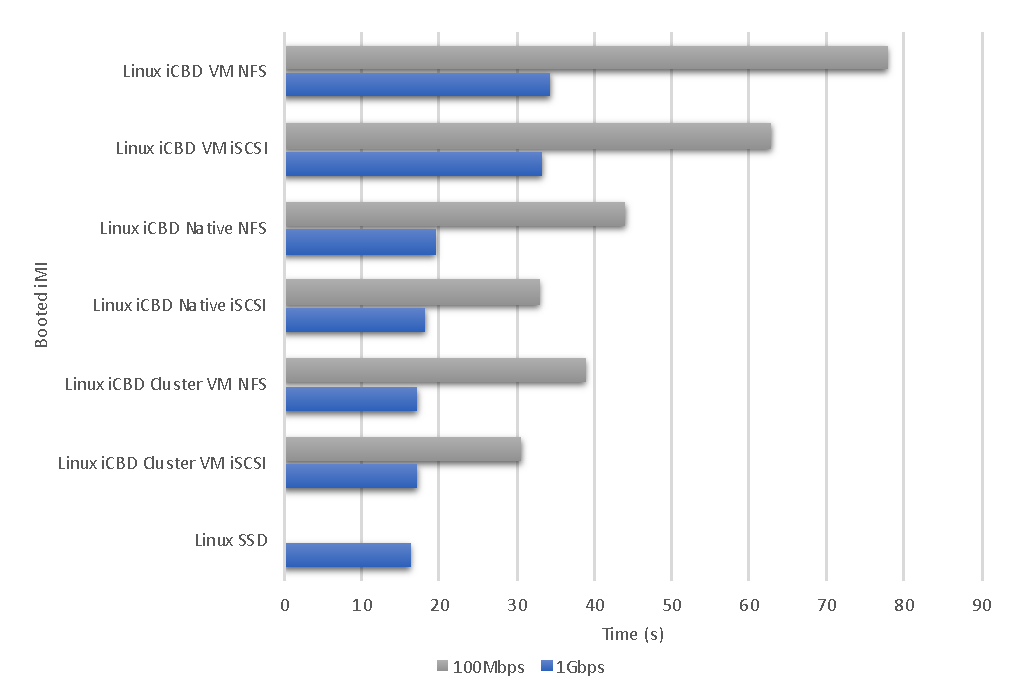
\includegraphics[height=4in]{cap5_secboot_cache}
	\caption{Boot time from iCBD-Cache02 in a five workstation sequential boot scenario}
	\label{fig:boot_cache}
\end{figure}

\begin{figure}[htbp]
	\centering
	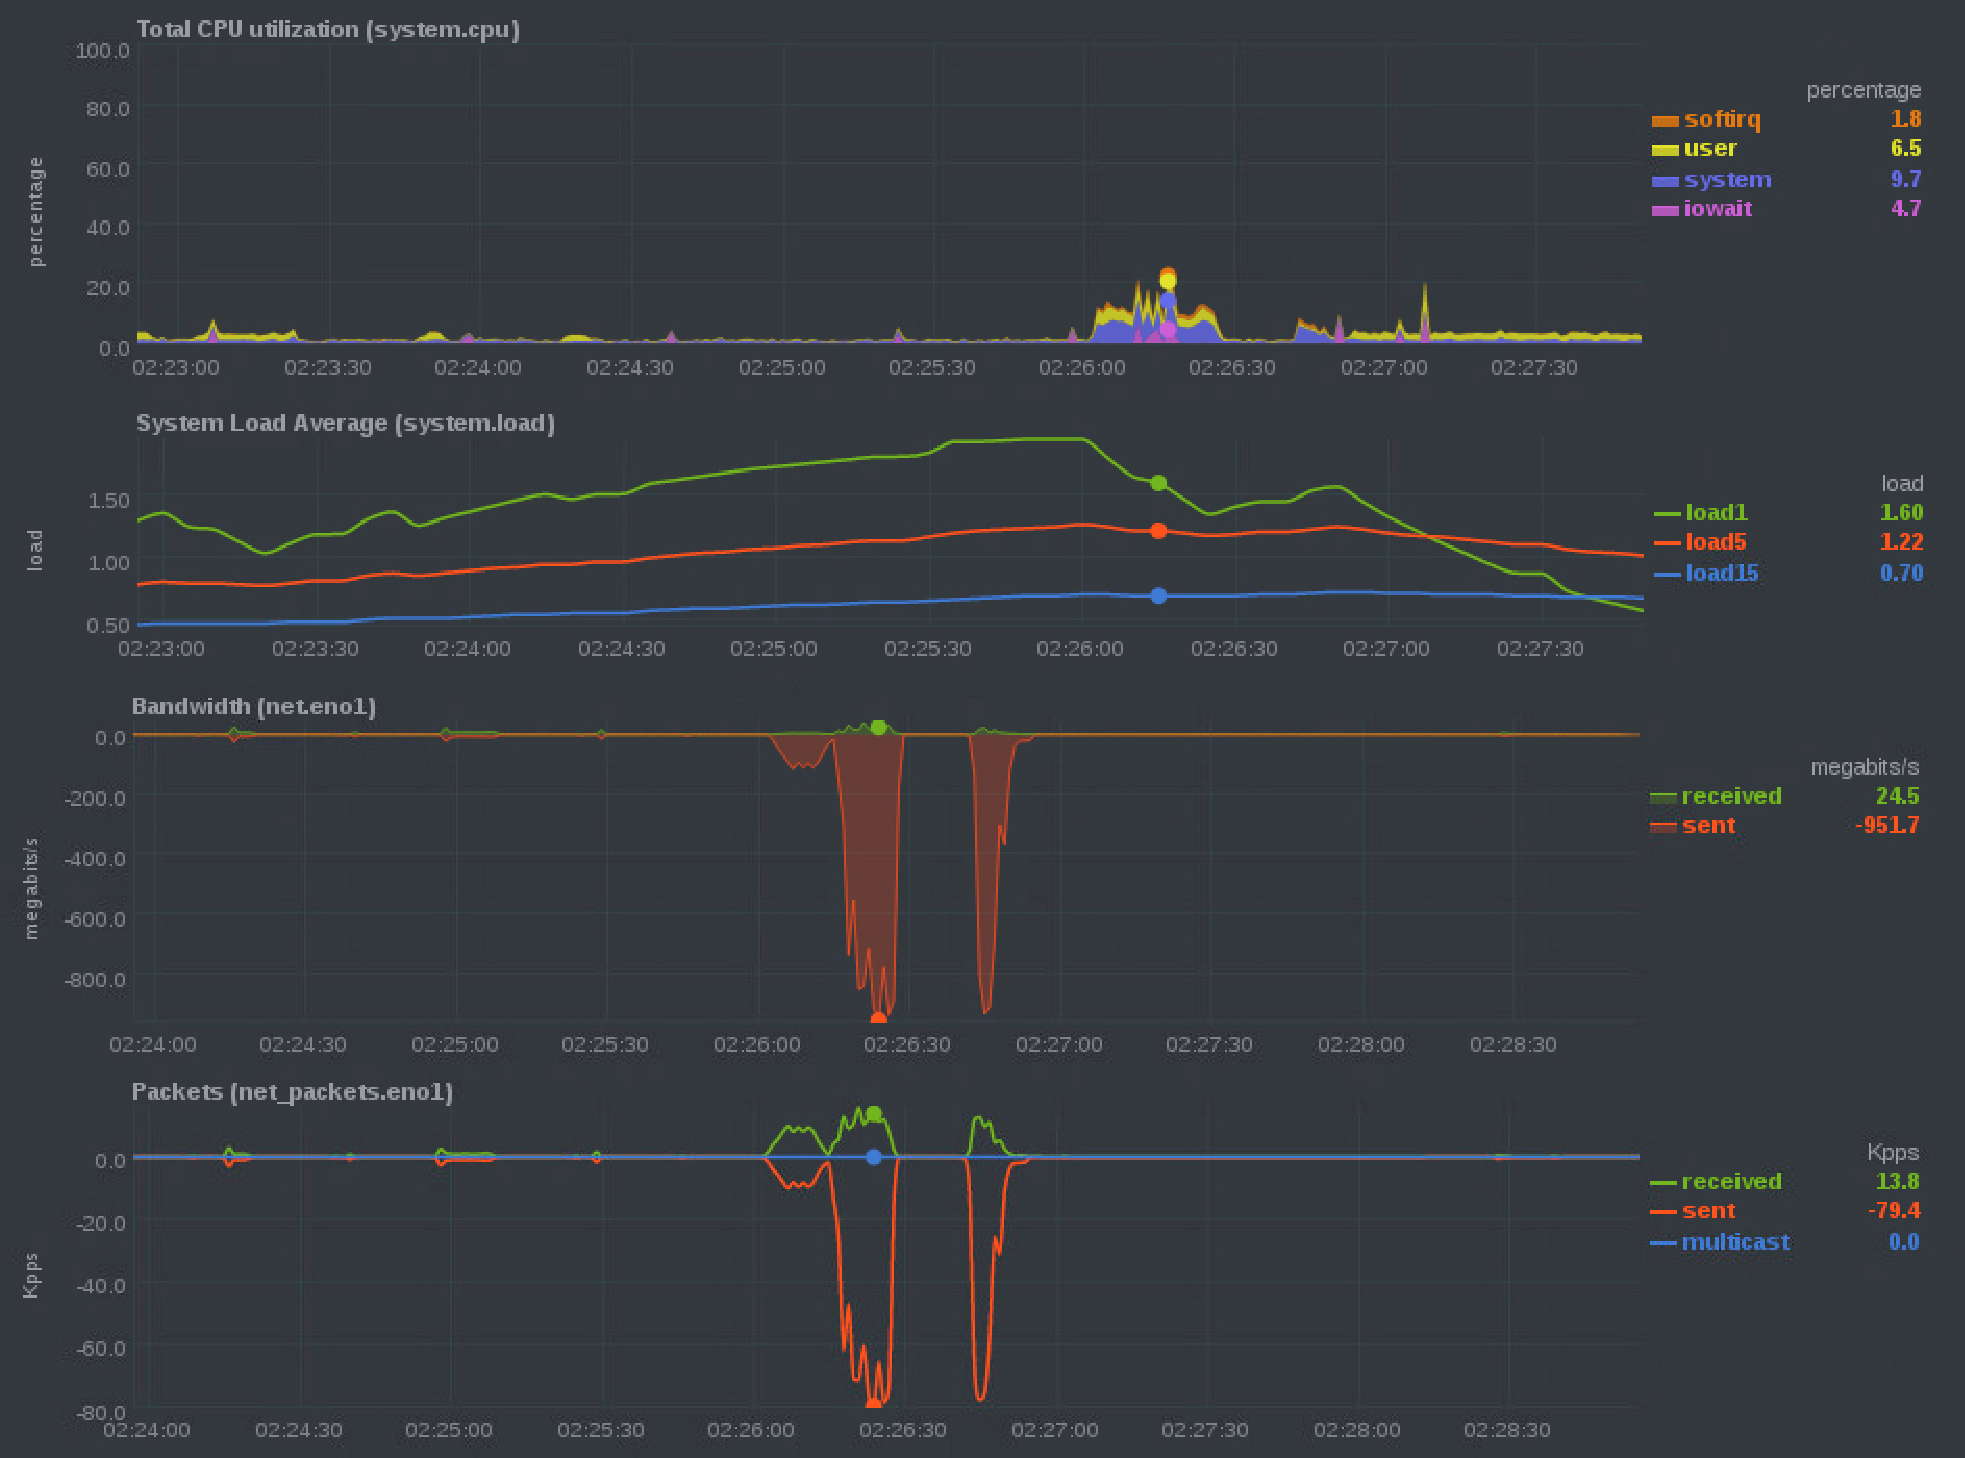
\includegraphics[height=4in]{cap5_secboot_cache_stats}
	\caption{System metrics for one run on the iCBD-Cache02 in a five workstation sequential boot scenario}
	\label{fig:boot_cache_stats}
\end{figure}

\begin{figure}[htbp]
	\centering
	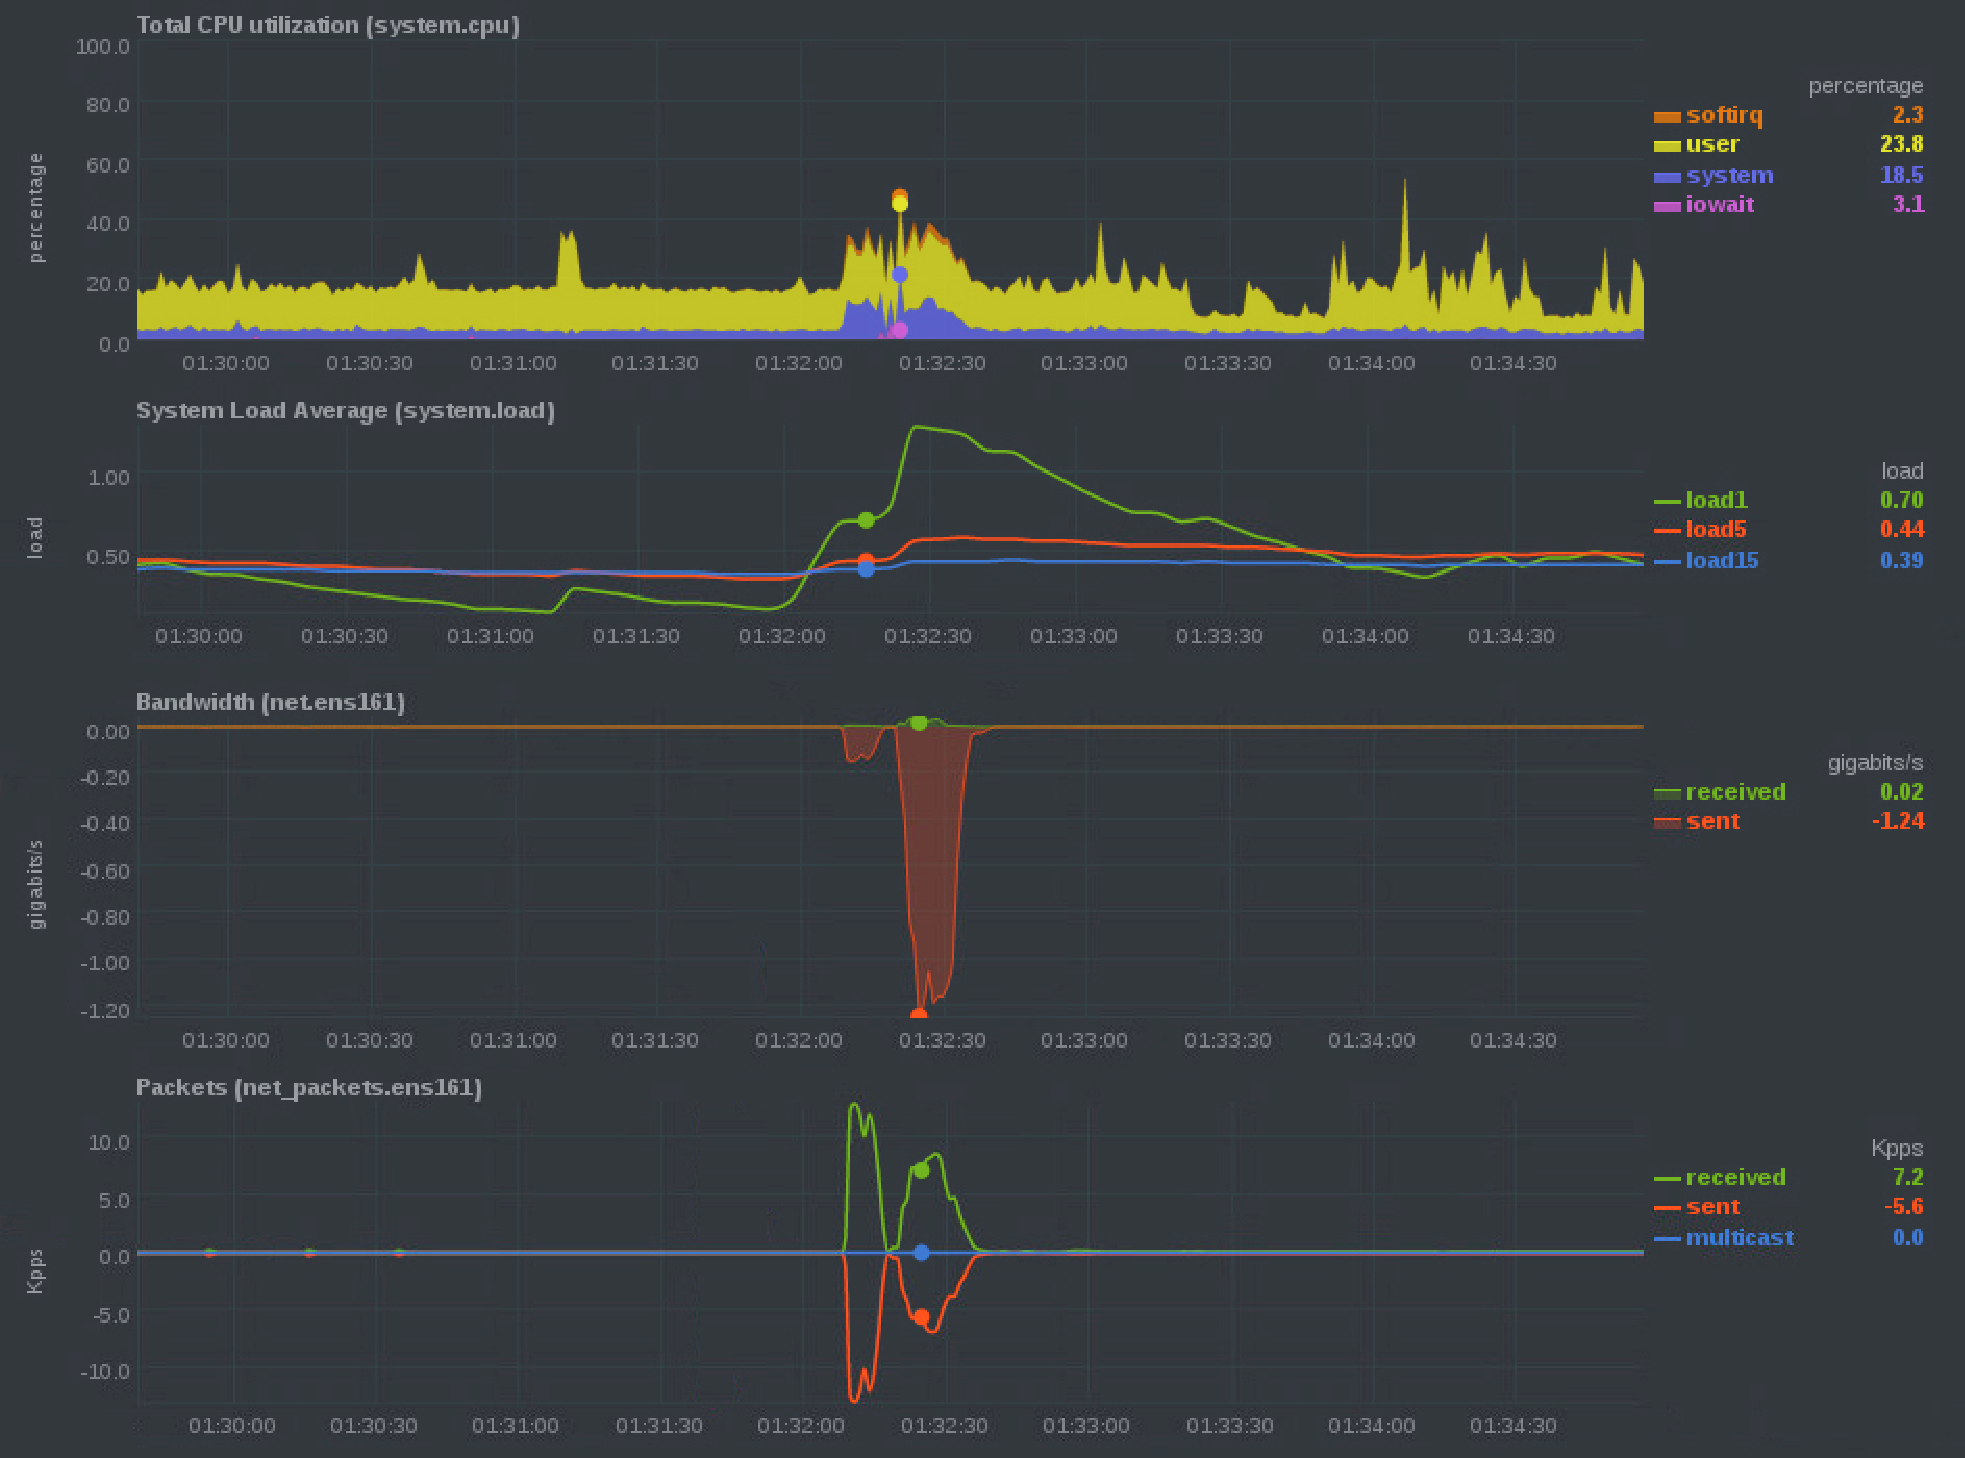
\includegraphics[height=4in]{cap5_secboot_imgs_stats}
	\caption{System metrics for one run on the iCBD-imgs in a five workstation sequential boot scenario}
	\label{fig:boot_imgs_stats}
\end{figure}

\begin{table}[]
\centering
\begin{tabular}{llcc}
\textbf{iMI} &  & \textbf{iCBD-imgs} & \textbf{iCBD-Cache02} \\ \hline
\multirow{2}{*}{\textit{Ubuntu 14.04 - Client Cluster}} & iSCSI & 453.5 MB & 454.3 MB \\
 & NFS & 703.0 MB & 702.1 MB \\ \hline
\multirow{2}{*}{\textit{Ubuntu 14.04 - Client Native}} & iSCSI & 456.3 MB & 453.6 MB \\
 & NFS & 704.2 MB & 703.8 MB \\ \hline
\multirow{2}{*}{\textit{Ubuntu 14.04 - Client VM}} & iSCSI & 834.1 MB & 836.8 MB \\
 & NFS & 950.5 MB & 952.8 MB
\end{tabular}
\caption{Total data received after booting, given each boot variant and for both iMI providers}
\label{tab:boot_totaldata}
\end{table}

\subsubsection{Benchmark in a Boot Storm condition}
\label{susub:eval_cache_bootstorm}

\begin{table}[]
\centering
\begin{tabular}{llcc}
\textbf{iMI} & \textbf{} & \textbf{iCBD-imgs} & \textbf{iCBD-Cache02} \\ \hline
\multirow{2}{*}{\textit{Linux iCBD Client Native}} & iSCSI & 20.035 s & 23.020 s \\
 & NFS & 23.248 s & 28.156 s \\ \hline
\multirow{2}{*}{\textit{Linux iCBD Client VM}} & iSCSI & 42.627 s & 46.752 s \\
 & NFS & 44.734 s & 53.840 s
\end{tabular}
	\caption{Comparison of boot times in a boot storm situation in both providers (iCBD-imgs and iCBD-cache02)}
	\label{tab:bootstorm_both}
\end{table}


\begin{figure}[htbp]
	\centering
	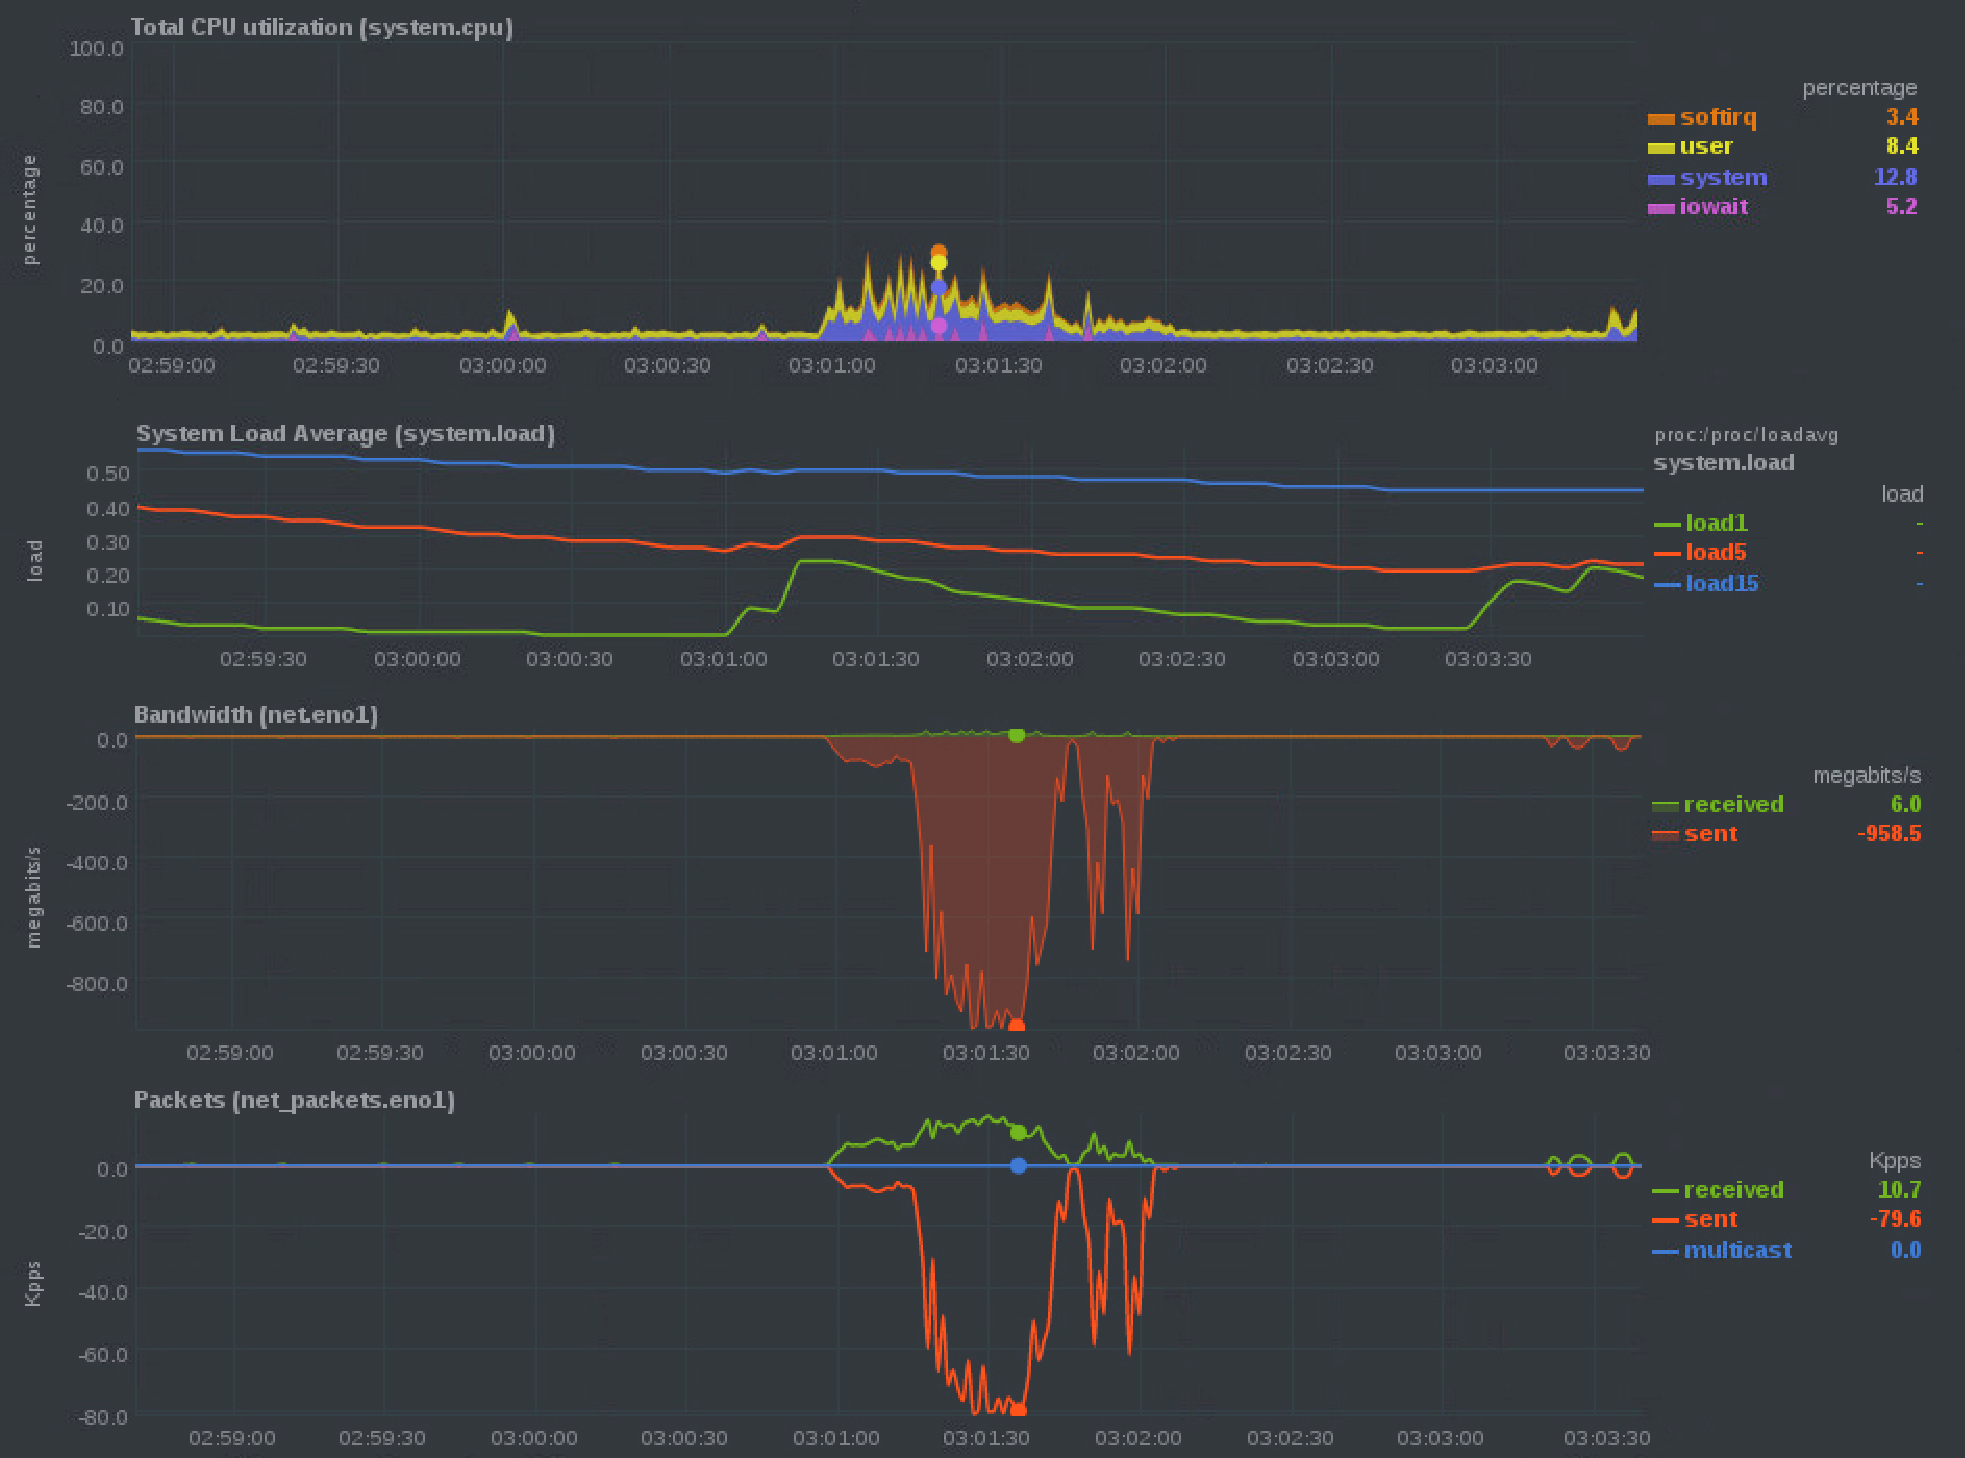
\includegraphics[height=4in]{cap5_bootstorm_cache_stats}
	\caption{System metrics for one run on the iCBD-Cache02 in a boot storm scenario}
	\label{fig:boot_cache_stats}
\end{figure}


%\textbf{TOPICS :}
%\begin{itemize}
%	\item benchmarking 
%	\item Boot time Lab PC
%	\item Boot time iCBD VM in Cluster
%	\item Boot time iCBD in Lab PC (100 / 1000 mbps) iCBD-Imgs VM
%	\item Boot time iCBD in Lab PC (100 / 1000 mbps) iCBD-Cache
%\end{itemize}